

\section{Theoretical Framework}

\begin{figure}[!htbp]
	\centering
		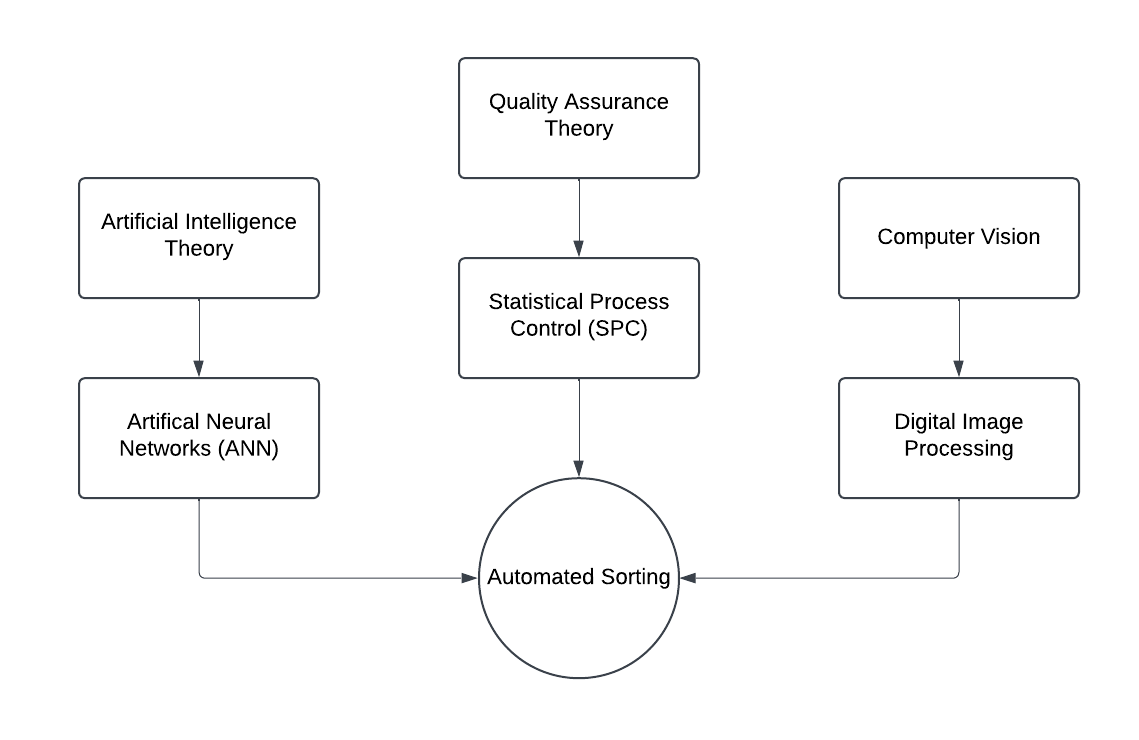
\includegraphics[width=0.8\textwidth]{figure/theoretical_framework.png}
	\caption{Theoretical Framework}
	\label{fig:theoretical_framework}
\end{figure}

The theoretical framework discusses the multiple concepts that are involved in this study. These key concepts are crucial to ensuring the success of the thesis. There are three main concepts that are key to this study, the Artificial Intelligence Theory, the Quality Assurance Theory and lastly, Computer Vision.

\section{Conceptual Framework}

\begin{figure}[!htbp]
	\centering
		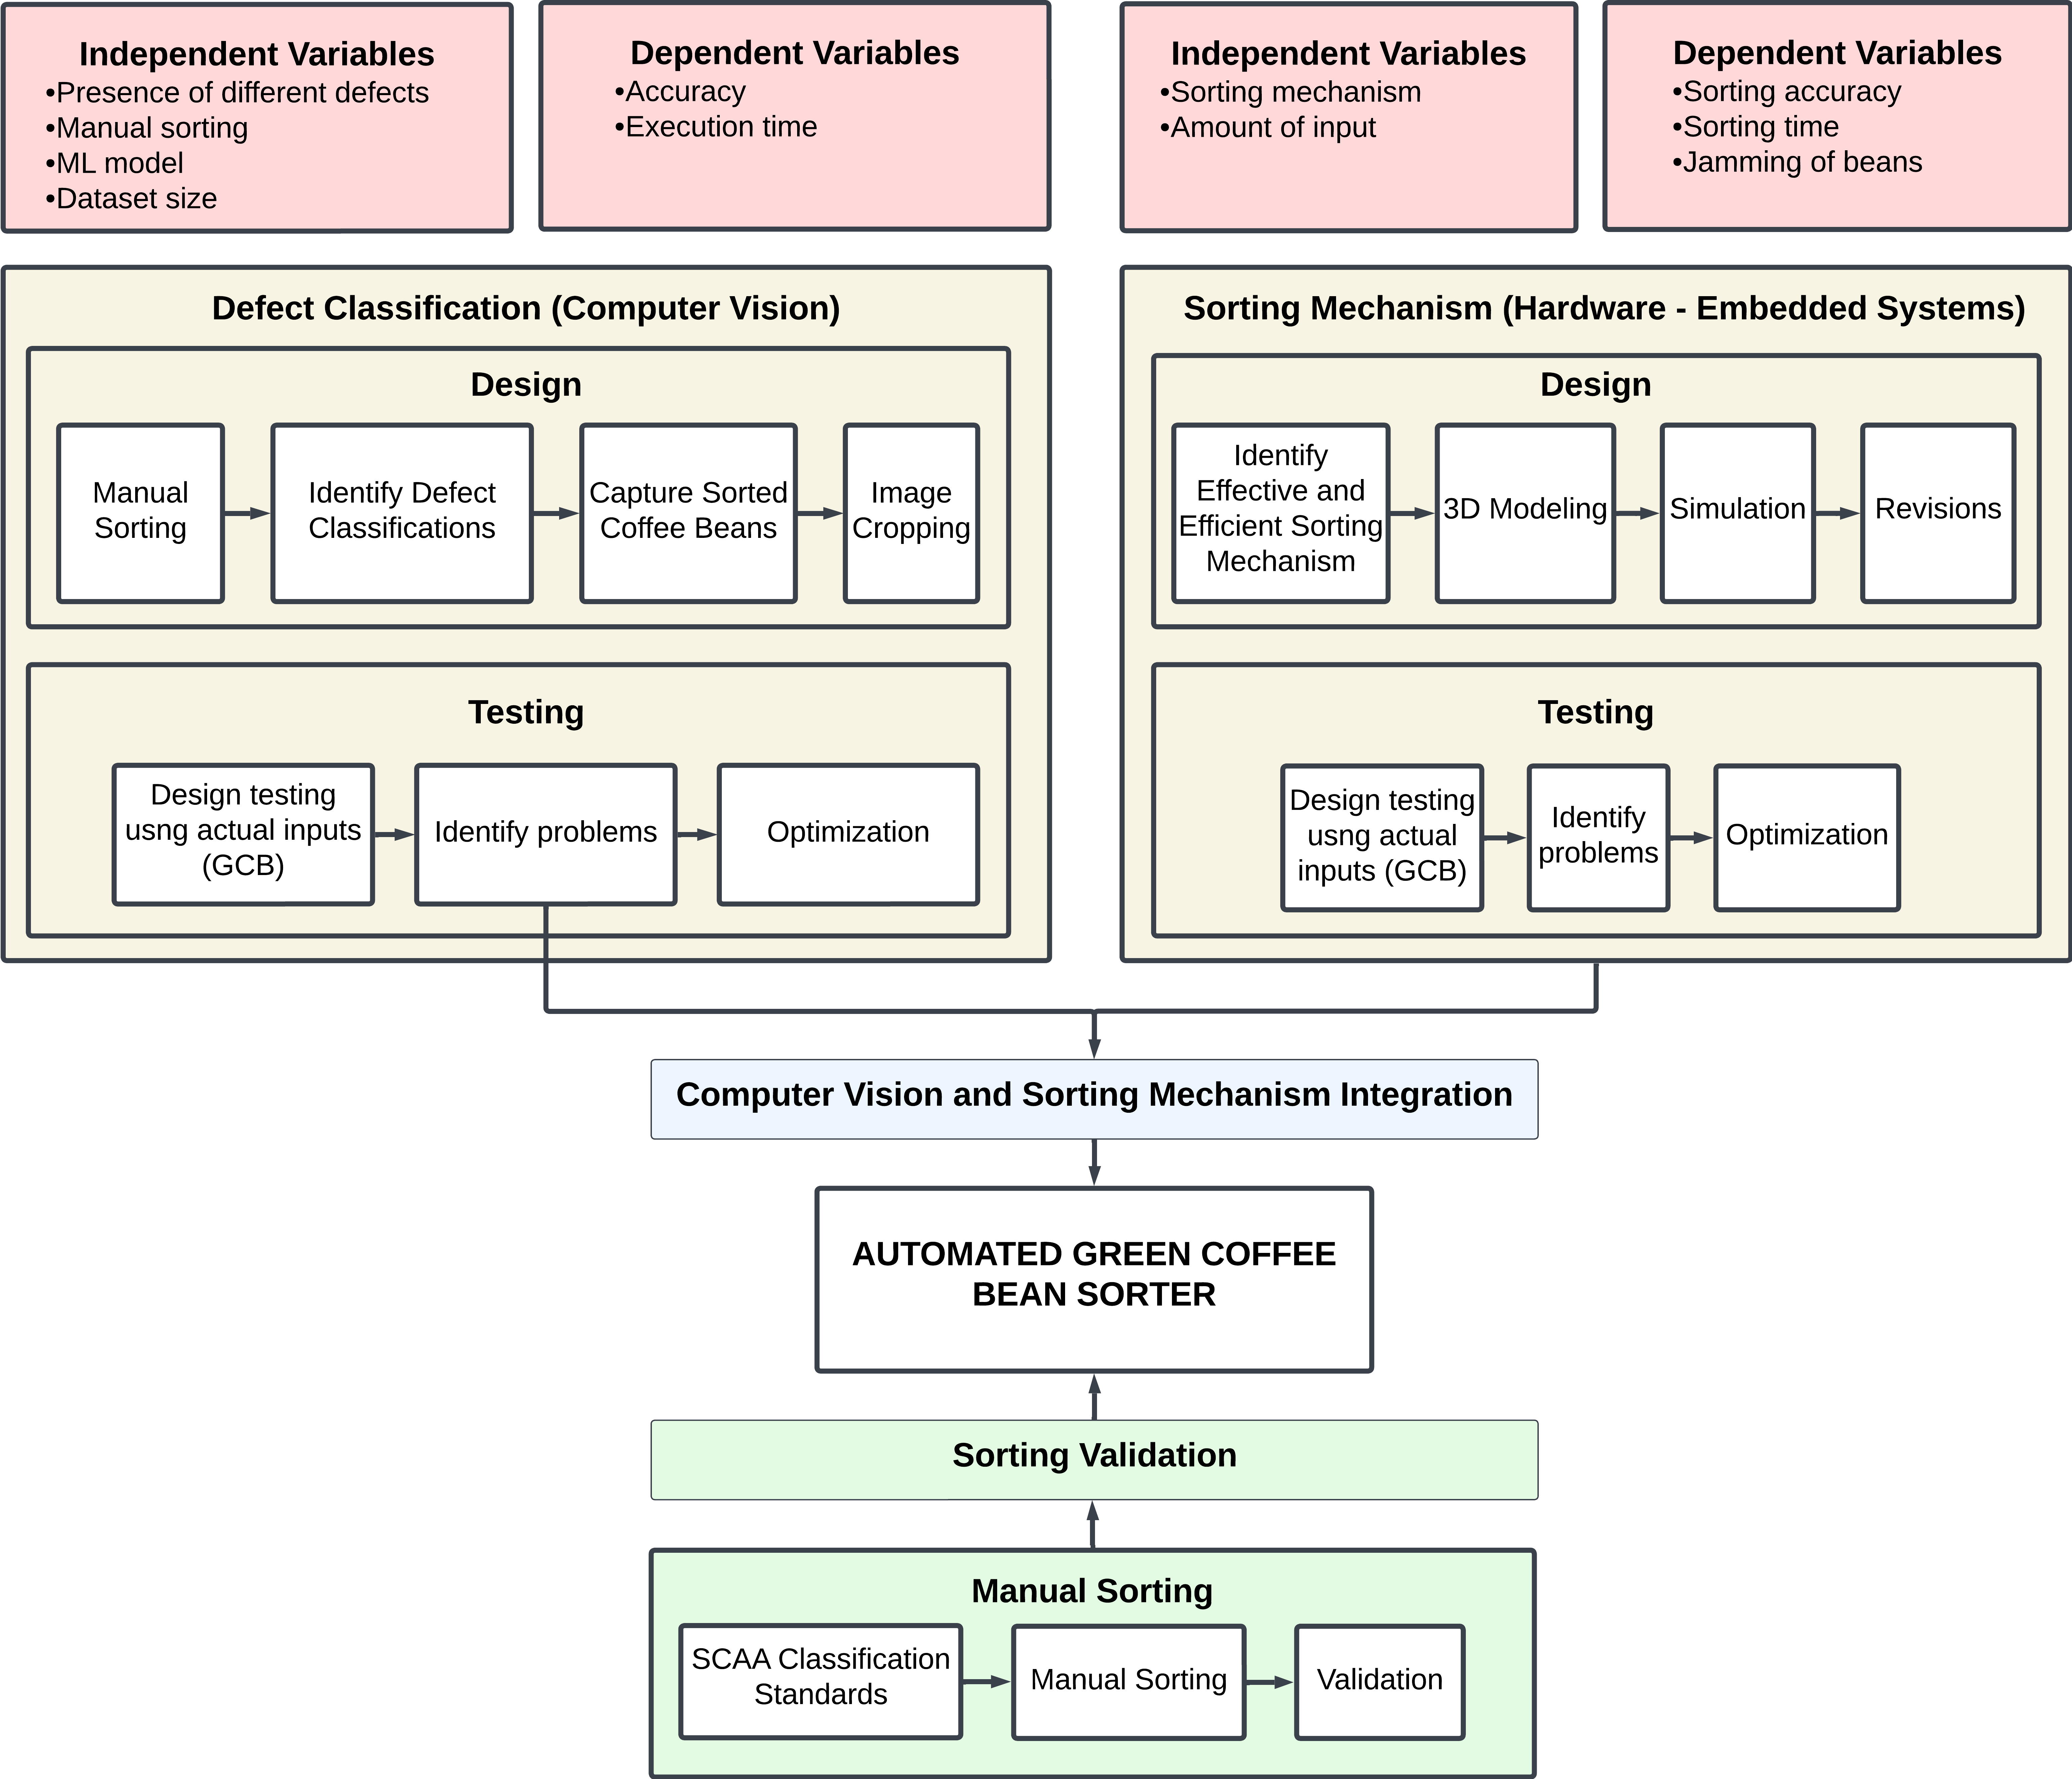
\includegraphics[width=\textwidth]{figure/conceptual_framework_v2.png}
	\caption{Conceptual Framework}
	\label{fig:conceptual_framework}
\end{figure}

The conceptual framework shows the implementation of two systems which consists of machine vision and embedded systems. The framework describes the thought process of both systems with the end goal of integrating both systems. The machine vision handles the defect classification of the system, whereas the embedded system handles the sorting of the beans. By integrating both systems together, creates an automated green coffee bean sorter. The data validation is done by sorting through the tested coffee beans by the system following the standards of the SCAA.

\section{Quality Assurance Theory}
Quality assurance theory refers to the set of principles and practices that focuses on establishing a systematic process to ensure that a product or service conforms to a predetermined standard. In the aspect of food and agriculture, there are a number of practices and principles that ensure the safety and quality of food products. According to \cite{da_Cruz_Cenci_Maia_2006}, there are a number of practices in place that must be followed, one of which is Good Agricultural Practices, where these procedures are aimed to reduce hazards related to product safety at the farm level. Another one of said practices is the Good manufacturing practice, which were formerly called support programs that provide foundations to the overall food safety management programme. This includes cleaning, maintenance, personnel training, calibration equipment, quality control, and  pest control. Industries that adopt such practices produce the following results, better quality products, greener initiatives and better productivity within a department. Lastly, hazard analysis and critical control points (HACCP), is a science-based system that was created to identify potential hazards and actions to control said hazards. This practice is used to ensure food safety. 

In the context of coffee beans, there are a number of systems in place to ensure that quality beans are being provided to the consumer market. The governing body known as the Specialty Coffee Association (SCAA) has implemented grades to green coffee beans to provide a better way to classify said beans. These grades can be differentiated into 5 grades namely, Specialty Grade, Premium Coffee Grade, Exchange Coffee Grade, Below Standard Coffee Grade, and Off grade Coffee. They are classified according to the number of defects found in a sample batch of 300 grams and according to their size. Specialty grade coffee beans are supposed to contain less than 5 defects in a sample batch while also not allowing any primary defects to be present; it should only have less than 5\% difference between its sizes. Coffee beans in this grade should also contain a special attribute whether in its body, flavor, aroma, or acidity, and its moisture content should only be in the range of 9-13\%. Premium Coffee grade beans should only contain 8 full defects in a sample batch but primary defects are allowed in the sample batch. Similarly to specialty grade coffee beans, its sizes should only contain a 5\% difference to one another; it should also contain a special attribute and moisture content should also be similar to its specialty grade counterpart. Exchange coffee grade should contain defects ranging from 9-23 beans in a sample batch, with sizes that can vary up to 50\% difference in weight but also only 5\% in its sizes. Below standard and off grade coffee beans are classified according to the number of defects present in a sample batch; 24-86 beans for below standard while more than 86 beans for off grade. These gradings are used to ensure that quality green coffee beans are produced and ensure that consumers are provided with the best quality available. 

\section{Artificial Intelligence Theory}

Artificial Intelligence in defect classification are widely used in this industry which are commonly used in manufacturing and industrial applications. Several deep learning techniques are used in order to achieve an effective defect classification. Models such as convolutional neural networks (CNNs)  and You Only Look Once (YOLO) are widely used for classification. CNN utilizes an image based analysis and feature extraction approach to identify different classifications. CNN is more effective in analyzing grid-like data like images, making it suitable for defect classification \cite{Das_Hollander_Suliman_2019}. One of its major advantages is its ability to automatically detect important features such as shape, patterns, and edges. Although it may have its own advantages, there are also disadvantages that need to be taken into account, mainly in scenarios that involve class imbalance and complex backgrounds (Moon, 2021) . YOLO is another model that is suitable for defect classification, its ability to provide real-time defect classification while also providing high accuracy is essential in some industries. In YOLO, there are several versions that are developed over the years, which are supposed to bring several improvements in terms of speed, accuracy, and computational efficiency. Combining different models is also effective, in the case of \cite{Deepti_Prabadevi_2024}, they combined transformer architecture with YOLOv7 to enhance its feature extraction, this resulted in an increase of 5.4\% in mean average precision and F1 score. 

\section{Computer Vision Theory}

There are fundamental concepts that need to be done for image processing in detection. There are pre-processing techniques like preprocessing and segmentation. Pre-processing is a general term for preparing an image to be analyzed by the system, this includes techniques such as denoising an image, applying filters, and enhancing the image to further improve the visibility of defects \cite{Lee_Tai_2020} . Segmentation is dividing the images into segments to make the analysis simpler, methods such as histogram segmentation and active contour models helps in isolating the regions of interest. 

For defect classification, feature extraction is important to identify the relevant features then extracting said features to to help indicate specific defects, this utilizes the edges, textures, and shapes to help in defect classification \cite{Wu_Hao_Song_2024}.  BY utilizing OpenCV and deep learning models is advisable for automatic feature extraction. Models like CNN, can automatically extract features from images, which greatly reduces the need for manual extraction, this helps in a more robust and scalable solution \cite{Bali_Tyagi_2020}. The versatility of OpenCV library which allows support for multiple image pre-processing tasks, when combined with deep learning models can be applied to different fields. 

\section{Performance Evaluation}

Accuracy, precision, recall, and F1 score are common measures to assess how well classification models predict. Accuracy measures how good a model is by computing the ratio of correct predictions to all predictions. While appropriate for balanced datasets, accuracy can be deceptive when dealing with imbalanced classes, since a model can be very accurate by predicting the majority class. Precision measures how well positive predictions are obtained by calculating the number of correct predicted positive instances. This is particularly important  when false positives are costly, such as in the case of spam. Recall, or sensitivity, measures how well a model identifies true positive instances, which is very important in cases where failing to detect a positive instance is costly, such as in medical diagnosis. Since precision and recall trade off each other, the F1 score reconciles the two by computing their harmonic mean. This measure is particularly appropriate when a trade-off between precision and recall is desired, so that neither false positives nor false negatives dominate the assessment. In general, these measures provide a general impression of how good a model is and help decide how well-suited the model is for different applications.

\section{Existing Technologies and Approaches}
The paper done by \cite{Lualhati_Mariano_Torres_Fenol_2022}, is a green coffee bean sorter that utilizes MATLAB as its image processing. The system created uses a PID based algorithm and image processing algorithm for sorting. The system utilized two cameras to capture both sides of the bean. The system of Lualhati et al. comprises only 3 green coffee bean classifications, which are good, black and deformed coffee beans. The developed system uses multiple stepper motors for the defect sorting, while 2 cameras were used to handle the green coffee bean detection. 

The paper of \cite{Balay_Cabrera_Jensen_Mayuga_2024}, is an automatic sorting for green coffee beans utilizing computer vision and machine learning for defect classification. The system developed uses the YOLOv8 model alongside a Raspberry Pi based image processing to identify and classify the green coffee beans. The defects that the group classified are full black, partial black, chipped, dried cherry, shell, and insect damage. The system developed uses a conveyor belt and sorting motor for an automated defect separation. They used one camera module, the raspberry pi camera module 3 NoIR for the defect detection of the system. 

\section{Density Measurement}
In measuring the density of the coffee bean there are a number ways this can be done, one way is by measuring the bulk density of the batch. This is done by measuring the mass of a batch then dividing it to a fixed volume. The more appropriate method for measuring the density of the coffee bean is called “free settle” density or free-flow density. This is defined as the ratio of the mass of the coffee beans to the volume they occupy after being allowed to flow freely into a container. It is expressed in grams per liter or kilograms per cubic meter. 

\begin{equation}
	d = \frac{m_2-m_1}{V}
\end{equation}

where $m_2$ is the mass of the green coffee bean, $m_1$ is the mass of the empty container, and $V$ is the capacity (in liters) of the container \cite{International_Organization_for_Standardization_1995}.

\section{Summary}
This chapter gives the theoretical and conceptual backgrounds of an automated green coffee bean sorter using Artificial Intelligence (AI), Quality Assurance, and Computer Vision. The theoretical background focuses on key concepts like deep learning models (CNNs, YOLO) used for defect classification, quality assurance principles (GAP, GMP, HACCP) ensuring food safety, and computer vision algorithms (preprocessing, segmentation, and feature extraction) used for image analysis. The conceptual background explains the integration of machine vision for defect detection with embedded systems for sorting, thus conforming to the SCAA coffee grading standards. Performance metrics like accuracy, precision, recall, and F1 score are used for evaluating the performance of the model. Current technologies, for instance, those of \cite{Lualhati_Mariano_Torres_Fenol_2022} and \cite{Balay_Cabrera_Jensen_Mayuga_2024}, provide insights relevant to image processing and machine learning-based sorting techniques, thus contributing to automated coffee bean classification development.
